%% LyX 2.0.6 created this file.  For more info, see http://www.lyx.org/.
%% Do not edit unless you really know what you are doing.
\documentclass[english]{article}
\usepackage[T1]{fontenc}
\usepackage[latin9]{inputenc}
\usepackage{color}
\usepackage{float}
\usepackage{amsmath}
\usepackage{graphicx}
\usepackage[numbers]{natbib}

\makeatletter

%%%%%%%%%%%%%%%%%%%%%%%%%%%%%% LyX specific LaTeX commands.
%% Because html converters don't know tabularnewline
\providecommand{\tabularnewline}{\\}

%%%%%%%%%%%%%%%%%%%%%%%%%%%%%% Textclass specific LaTeX commands.
\newenvironment{lyxlist}[1]
{\begin{list}{}
{\settowidth{\labelwidth}{#1}
 \setlength{\leftmargin}{\labelwidth}
 \addtolength{\leftmargin}{\labelsep}
 \renewcommand{\makelabel}[1]{##1\hfil}}}
{\end{list}}

\makeatother

\usepackage{babel}
\begin{document}

\title{Interactive Visualization on Temporal and Longitudinal Data}

\maketitle

\section{Overview}

Any interactive visualization is built upon the static graphs. Interactions
would change the static pictures by some order such that the user
can find the best graphical summary. Hence before introducing the
interactive graphics, we give an overview of the static graphics for
temporal and longitudinal data in this section.


\subsection{Time-dependent data}

Time-dependent data could be complex due to many factors, like the
time formats (year/month/week/day/hour/minute/second/...), data types(discrete
or continuous, events or intervals, etc.), dependent variables, and
so on. The custom time formats brings some further problems, for example,
the number of weeks per year is not an integer, the number of days
per month varies over the year, and the leap year recurs every four
years. In some cases, the data can only be collected during the weekdays.
Therefore, the time plot may not be accurate in an absolute time line,
and the length of the periodicity could be hard to verify. Besides,
the dependent variables could appear with different time formats,
which makes the visualization more difficult but interesting.

The main division of the data types is that whether the time is discrete
or continuous. For example, the time to record the salary of an employee
is discrete, but the time for the temperature in a location is continuous.
However, people can not measure a variable continuously over time,
so the data collected is still discrete. To simplify the problem,
we only consider the discrete case. Another further division of the
discrete time series data is that whether a time datum is recorded
as an event or an interval. For example, in a customer visiting problem,
the time length that each customer stays (interval) is as important
as the time that the customer enters (event). Again, to simplify,
we only consider the event type. 

Now we will have two situations: regular time spacing and irregular
time spacing. Regular time spacing means that the measurement happens
successively with a constant time space. Irregular time spacing could
arise from the missing values of regular time spacing, or the varying
time interval. Figure \ref{fig:Time-series-plots} shows the two situations.

\begin{center}
\begin{figure}[h]
\begin{centering}
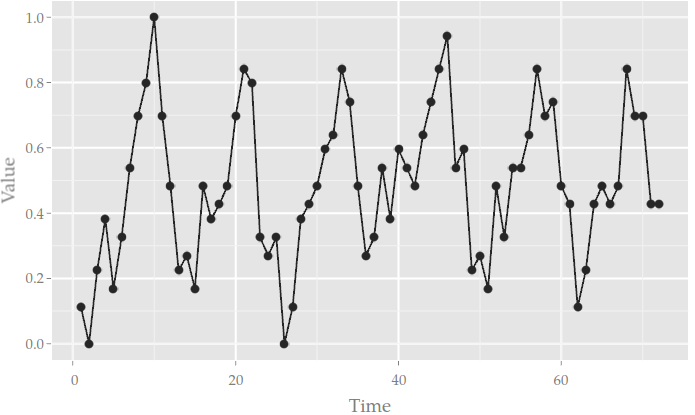
\includegraphics[width=0.48\textwidth]{graph/pipeline-01-1} 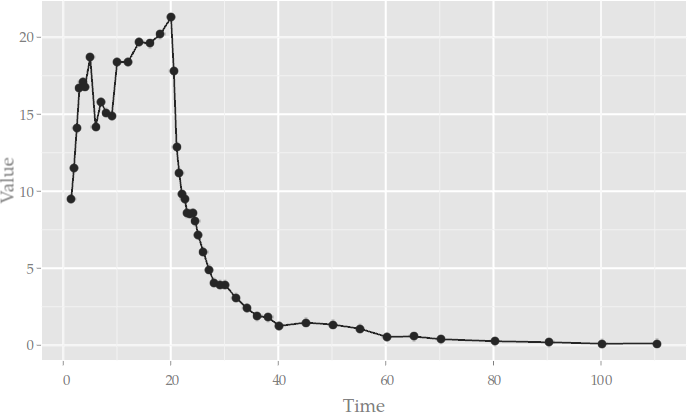
\includegraphics[width=0.48\textwidth]{graph/pipeline-02-1}
\par\end{centering}

\caption{\label{fig:Time-series-plots}Time series plots for regular time spacing
(left) and irregular time spacing (right).}
\end{figure}

\par\end{center}

Visualizing the longitudinal data is another challenge to the time
plots. It brings some issues, such as (1) intensive layout for a relatively
large number%
\footnote{20 can be considered as a large number for the graphical layout.%
} of individuals, (2) a few overwhelming large representatives could
make the other individuals invisible, (3) comparison between two or
more individuals is difficult if they are not plotted closely.


\subsection{Time visualization}

The common factor in the temporal and longitudinal data plots is the
time, and the different ways to orient time as the axis classifies
the graphs into different groups as follows.
\begin{enumerate}
\item Time on the horizontal axis

\begin{itemize}
\item Line graphs. Figure \ref{fig:Time-series-plots} gives two examples
for the univariate time series. For the longitudinal data, a simple
line graph is like Figure \ref{fig:Line-graph}.


\begin{center}
\begin{figure}[h]
\begin{centering}
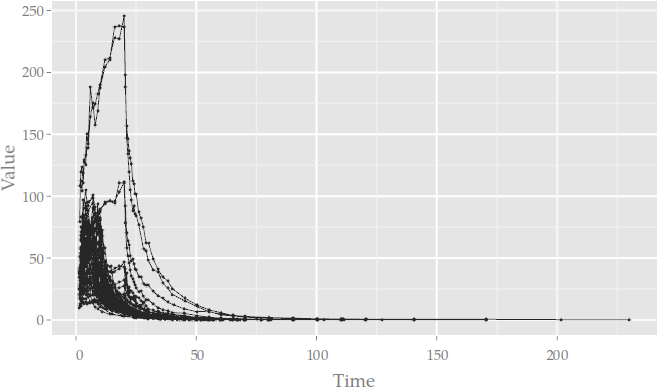
\includegraphics[width=0.6\textwidth]{graph/pipeline-03-1}
\par\end{centering}

\caption{\label{fig:Line-graph}Line graph for the longitudinal data.}
\end{figure}

\par\end{center}

\item Small multiples. Widely used for ages but summarized and introduced
by \citet{tufte1983visual,tufte1991envisioning}, the small multiples
display the data in multiple images. For multiple time series, including
the multivariate and longitudinal data, the graphical space is split
by the series.
\item Stacked graphs. Originated by \citeauthor{playfair2005playfair} in
1700's and recently discussed by \citet{byron2008stacked,javed2010graphical,heer2010tour},
a stacked graph draws the time series sequentially, and uses the previous
time series as the baseline for the current series. It is mostly used
for the longitudinal data rather than multivariate time series since
the individuals from the longitudinal data share the same scale.
\item Themeriver and streamgraph. Themeriver is created by \citet{havre2000themeriver},
which is a special case of the stacked graphs, since it moves the
starting baseline from the bottom to the center, and makes the plot
symmetric vertically. Streamgraph is developed later by \citet{byron2008stacked}.
It changed the algorithm to avoid the symmetry which increases the
internal distortion.
\item Horizon graphs. The horizon graph is inspired by two-tone pseudo coloring
\citep{saito2005two} and formally developed at Panopticon Software
\citep{reijner2008development}. Two-tone pseudo coloring is a technique
to visualize the details of multiple time series precisely and effectively.
However, the horizon graph became more popular after mirroring the
lower part of the series and simplifying the color scheme. The horizon
graphs were designed for visualizing the stock prices and economic/financial
data, so the features fit the requirements very well: (1) The data
have a baseline, which is usually the value at the starting time point.
Then the baseline can be used to mirror the negative part to the positive,
in order to save the graph space, where `negative/positive' means
smaller/greater than the baseline. (2) The positive and negative performance
should be distinguished, so the horizon graph provides two hues. (3)
The number of the color bands should be small, usually three color
bands for the positive values and three for the negative. Finding
the band height is easy for the stock prices since they can use 10\%
of the initial value, and in most cases the price will not increase
or decrease for more than 30\%.
\end{itemize}
\item Time on both horizontal and vertical axes

\begin{itemize}
\item Calendar heat maps. The idea of using two axes for the time is not
new. \citet{keller1993visual} used days and hours on two axes. \citet{van1999cluster}
proposed a colored calendar visualization (weeks and days on two axes).
\texttt{\textbf{d3.js}} \citep{bostock2012data} applies the calendar
heat maps and makes it interactive.
\end{itemize}
\item Time in the polar coordinates

\begin{itemize}
\item Nightingale's coxcomb. Florence Nightingale might be the earliest
author of a time series plot in polar coordinates. In the original
plots, two unstacked barcharts were made in polar coordinates. Each
diagram represents for one year. Later, people use the Nightingale's
coxcomb \citep{nightingale1858notes}, also called circular histogram
or rose diagram \citep{nemec1988shape}, to plot the time series with
a regular period like year or day.
\item Spiral graphs. This approach is proposed by \citet{weber2001visualizing}.
It can be seen as a temporal heatmap in polar coordinates. This approach
is good for seeking the period, but the length for the same time unit
changes over the loops. Besides, spiral graphs would be unhandy for
the short period problems and multiple time series.
\end{itemize}
\end{enumerate}

\subsection{Types of interactions\label{sec:Types-of-interactions}}

Different from the dynamic graphics, which arranges the visible graphics
change prior to the plotting step, and not allows the user to play
with any further interaction, interactive graphics emphasize the user
manipulation via the input device like the keyboard and mouse \citep{symanzik2012interactive}.
\citet{swayne1999} also explained the idea of interactive graphics:
it may imply the direct manipulation of the graph itself, manipulation
of the graph controls, or even the command-line interaction with graphs.
\citet{xie2014reactive} provided a classification to the interactions,
which depends on where the interaction happens. Two types are mentioned
in the article: single display interactions and the linking between
different displays. Single display interactions include many different
interactions, such as brushing, zooming, panning, querying, etc. Linking
between different displays connects multiple graphic windows via brushing.
The graphs could be either the same type, or different types, like
the scatterplot, histogram, map, etc. The paper also refers a list
of software for each type.

From another angle, the interactions can be classified by complexity:
\begin{itemize}
\item Human command. This is a one-way, direct manipulation that the user
asks the computer to execute immediately. For example, with a graphical
user interface (GUI), we can change the graph parameters simply by
clicking a button. Another example is querying. \citet{theus2011interactive}
gave a well description on how to query the information, where the
``command'' is pausing the mouse icon on an object. This type of
interactions does not require a following command, usually one single
command can achieve the goal.
\item Human-computer cooperation. Sometimes a single manipulation cannot
give a satisfactory result. For example, to explore the features of
a set of variables conditional on another set of variables, brushing
on a fixed area is not enough. We may need to move the brush from
one side to the other side of the conditional variables, to detect
the trend of interest. And if needed, we may change the brush size,
or select the union of some separate areas. It is usually a series
of continual manipulations, based on the instant computer output.
Hence we call this bidirectional type to be the human-computer cooperation.
\end{itemize}
The programming complexity for two types differs much. The unidirectional
human command works as long as a function is attached to the action
as a handler. The result need not to be saved since usually no following
commands are executed on the result. In contrast, human-computer cooperation
requires the accessibility to the result at any time, to prepare for
the next command. This feature of human-computer cooperation brings
at least two issues: rewritability of the result storage, and accessibility
from different function environments to the result. \citet{xie2014reactive}
answered the second question based on the design of \texttt{\textbf{cranvas}}\citep{cranvas}.
This paper will discuss the first question in Section \ref{sec:Pipeline}
and the second question from the aspect of linking in Section \ref{sec:Linking}.
Before that, we need to introduce the plot regions of interactions
in Section \ref{sec:graph-layers} and the design of interactions
in Section \ref{sec:Design-of-interactions}, because the instructions
will make the following discussion clear.


\section{Graph layers\label{sec:graph-layers}}

A well-defined plot region is the base of any visualization. For the
interactive graphics, different layers are desired as the plot regions
by different interactions. Usually there are many layers for an interactive
graph, because a complex interaction can be then decomposed into small
simple tasks on different layers. One layer is often designed for
only one graph element, like the title layer, x-axis layer, or brush
layer. Based on the characteristics of the graph elements, different
painting functions are used to make the plotting fast for layers.
When one layer changes, the irrelevant layers will remain the same.

\begin{center}
\begin{table}[h]
\begin{centering}
\begin{tabular}{c|c|c}
\hline 
common & required & brush, identify, keys\tabularnewline
\cline{2-3} 
layers & optional & grid, x-axis, y-axis, x-label, y-label, title \tabularnewline
\hline 
 & scatterplot & point\tabularnewline
\cline{2-3} 
special & histogram & bar, cue\tabularnewline
\cline{2-3} 
layers & map & polygon, googlemaps, path, point\tabularnewline
\cline{2-3} 
 & time plot & point, line, area, stats\tabularnewline
\hline 
\end{tabular}
\par\end{centering}

\caption{\label{tab:Layers}Common layers for all graphs and special layers
for four graph types in \texttt{\textbf{cranvas}}.}
\end{table}

\par\end{center}

In \texttt{\textbf{cranvas}}, about ten layers are used for each graph
type. Table \ref{tab:Layers} lists the layers for a few graph types
as an example.

To visualize time-dependent data, we should consider three basic layers:
point layer, line layer, and area layer (Figure \ref{fig:three-layers}).
Three painting functions will call three types of data input for the
three layers. The coordinates of the points are initially adopted
from the data, then the interactions may change the locations of the
dots. Then, the line layer connect the current positions of the points,
so it requires the order, or say, path information, which means that
for each point, the previous and next points are known. At last, the
area layer shades the area under the line by rendering a sequence
of polygons. Note that the baseline of the area need to be calculated
from the data. Figure \ref{fig:layer-system} shows the relationship
among three layers. 

\begin{center}
\begin{figure}[h]
\begin{centering}
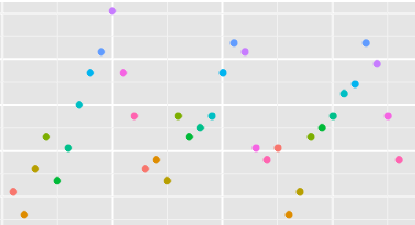
\includegraphics[width=0.32\textwidth]{graph/pipeline-11-point} 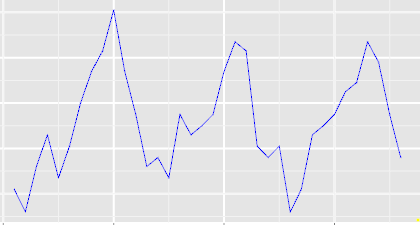
\includegraphics[width=0.32\textwidth]{graph/pipeline-11-line}
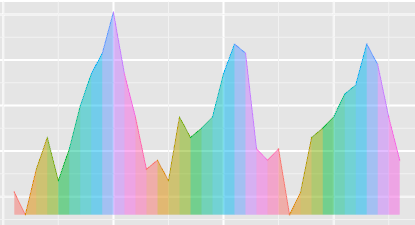
\includegraphics[width=0.32\textwidth]{graph/pipeline-11-area}
\par\end{centering}

\caption{\label{fig:three-layers}From left to right: point, line, and area
layers for the same data.}
\end{figure}

\par\end{center}

\begin{center}
\begin{figure}[h]
\begin{centering}
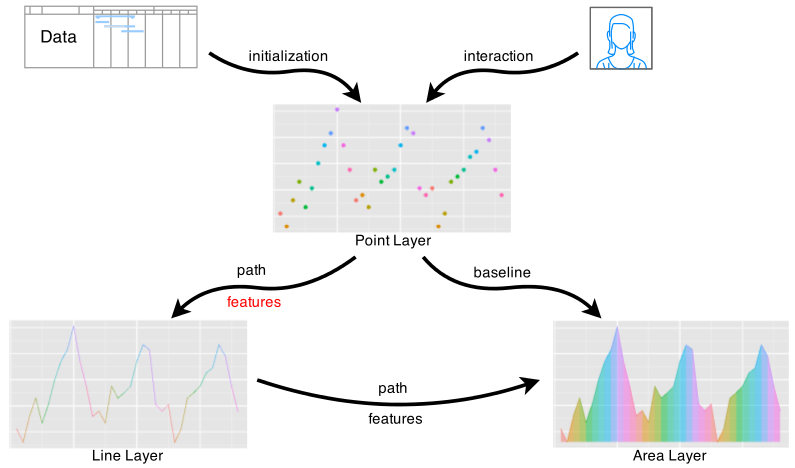
\includegraphics[width=0.8\textwidth]{graph/pipeline-12-threelayers}
\par\end{centering}

\caption{\label{fig:layer-system}The point layer is the center of the system
that receives the data and interactions at first. Then the line and
area layers adopt the current position from the point layer.}
\end{figure}

\par\end{center}

There are two remarks in the layer system for interactive time plots. 
\begin{enumerate}
\item Transmission of the painting features. Based on the setting of \texttt{\textbf{cranvas}},
the painting features like color, size, or visibility, are generated
for each observation when creating the mutaframe\citep{plumbr2014,xie2014reactive}.
As discussed above, the initial input in the time plots, are the points,
which means \texttt{\textbf{cranvas}} produces the painting features
for each point. \\
However, the number of points are not the same as the number of edges%
\footnote{One edge connects two points.%
}, because for each line, 
\[
\#\, of\, points=\#\, of\, edges+1;
\]
and for a time plot with $n$ series, 
\begin{equation}
\#\, of\, points=\#\, of\, edges+n.\label{eq:points_edges}
\end{equation}
Similarly, in an area layer, each polygon is defined by two adjacent
points, or, one edge, i.e., 
\[
\#\, of\, polygons=\#\, of\, edges.
\]
Now the problem is, how to get the painting features for each edge
and polygon? It is easy to answer the question when the features of
points are identical. But when they are varied, we have to skip the
features of $n$ points for $n$ lines by Equation (\ref{eq:points_edges}).
Then how to choose the $n$ points? One possible but not perfect solution
is the first or last point of a line, like shown in Figure \ref{fig:features}.
A smoother method should be considered for the edges and polygons
that connect two points with different features. To make it convenient
for the interactions, the method should be simple and avoid involving
new coordinates.\\
\begin{figure}[h]
\begin{centering}
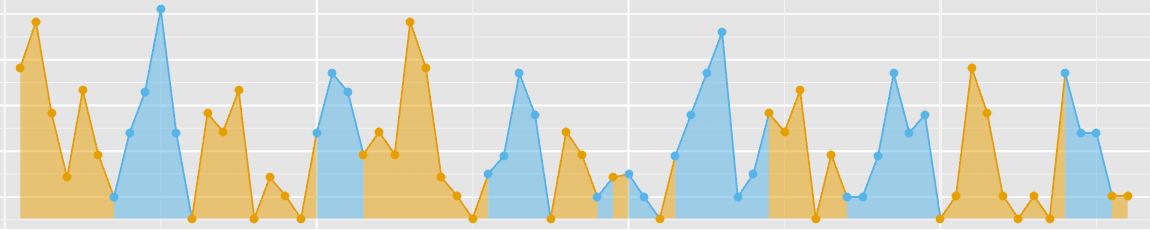
\includegraphics[width=0.9\textwidth]{graph/pipeline-13-layer-features}
\par\end{centering}

\caption{\label{fig:features}The colors of points are different, so the colors
of the edges and polygons follow the points ahead in this case.}
\end{figure}

\item Additional coordinates for the area layer. The point layer only needs
the x-y coordinates, while the line layer needs the x-y coordinates
in order and in group for lining up. But the area layer needs more
-- the baseline, which should be generated by variable%
\footnote{A variable or series may consist of several lines.%
}. When the y-coordinates of the variable change, like the shifting
in section \ref{sub:Special-interactions}, the baseline need to be
updated instantly. The additional information challenges the linking
system, and some details are discussed in Section \ref{sub:Linking-of-the-addition}.
\end{enumerate}

\section{Interactivity\label{sec:Design-of-interactions}}

For the time-dependent plots, \citet{wills2012visualizing} summarized
the interactivity from two aspects: parameters and data. On one hand,
the parameters are modified for the purpose of changing the element,
aesthetic, coordinate, statistic, scale, facet, or transform, while
the data remain the same. On the other hand, to brush, link, or drill-down(zoom-in),
the data are modified -- not necessarily the positional information,
but also the augmented variables used in the display. However, some
of the ideas for the parameters are conceptual and there is no software
to integrate them all.

In reality, the interactions like brushing, selection, linking, zooming,
panning, and querying, were already embedded in some interactive graphics
software. \texttt{\textbf{Prim-9}}\citep{fisherkeller1988prim}, \texttt{\textbf{Diamond
Fast}} \citep{unwin1988eyeballing}, \texttt{\textbf{XQz}}\citep{McDougall1994},
\texttt{\textbf{XGobi}}\citep{swayne1998xgobi}, \texttt{\textbf{GGobi}}\citep{cook2007ggobi},
\texttt{\textbf{Fortune}}\citep{kotterfortune}, \texttt{\textbf{TraXplorer}}\citep{Javed2010},
\texttt{\textbf{d3.js}}\citep{bostock2012data}, and \texttt{\textbf{cranvas}}\citep{cranvas}
used some or all of the interactions.

Within the realized interactions mentioned above, all but querying
belong to the human-computer cooperation, based on the discussion
in Section \ref{sec:Types-of-interactions}. For more explanation,
brushing requires the knowledge of the current brush location, and
returns the corresponding brushed points. Selection hears from the
selection methods, the current selected points, and the cursor location,
to return the new selected points. Linking transmits the brushed status
from one graph object to another. Zooming and panning uses the current
cursor location and zooming range to anchor the new range. All of
these returned objects or status should be saved for future use. Hence,
the strength of the above software is to support the instantly data
exploration conveniently, compared to other interactive tools like
GUI. 

Note that these interactions (brushing, selection, linking, zooming,
panning, querying, etc.) are universal for all graph types. Considering
the unusual characteristics of the temporal and longitudinal data,
some special interactions should be utilized to reveal the time-dependent
structure and series associations easily and quickly. In this section
we introduce the design of the interactions and discuss the the interactivity
issues.


\subsection{Design\label{sub:Special-interactions}}
\begin{itemize}
\item Switching between layers.


Starting from the basic demand, the interactive time plots should
support the switch between the line and area layers, as the line and
area plots have their own pluses and minuses. The line plots are concise
when comparing the series in the same scales, in contrast the area
plots make the space noisy with the overlapping area. As shown in
Figure \ref{fig:switching-layers}(1), the area draws much attention
but not necessary. In some other cases like the small multiples, the
area plots are better because when the baselines are not of the same
height, the area makes the understanding and comparison more accurate
between values from different series. In Figure \ref{fig:switching-layers}(2),
the line plot does not deliver the information as clearly as the area
plot, on the overall high values of series B1 and low values of series
A1.


\begin{figure}[h]
\begin{centering}
\begin{tabular}{cc}
\multicolumn{2}{c}{{\scriptsize{(1) Line plot is better than the area plot.}}}\tabularnewline
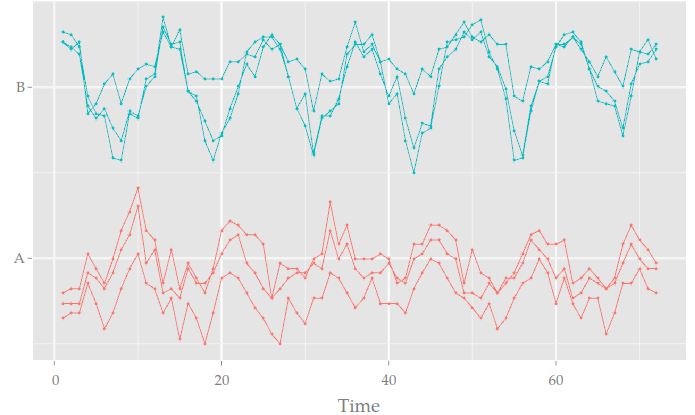
\includegraphics[width=0.48\textwidth]{graph/pipeline-14-6} & 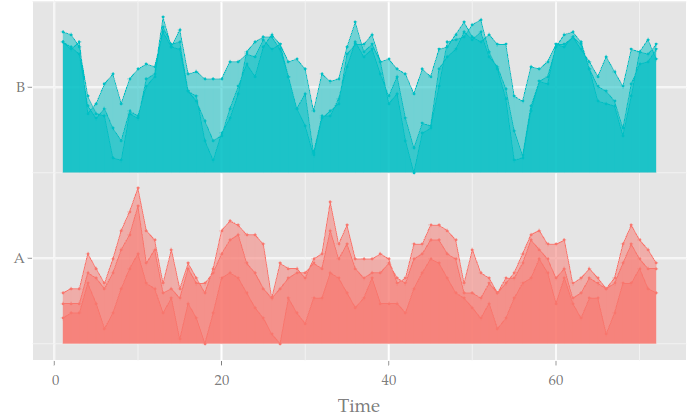
\includegraphics[width=0.48\textwidth]{graph/pipeline-14-8}\tabularnewline
 & \tabularnewline
\multicolumn{2}{c}{{\scriptsize{(2) Area plot is better than the line plot.}}}\tabularnewline
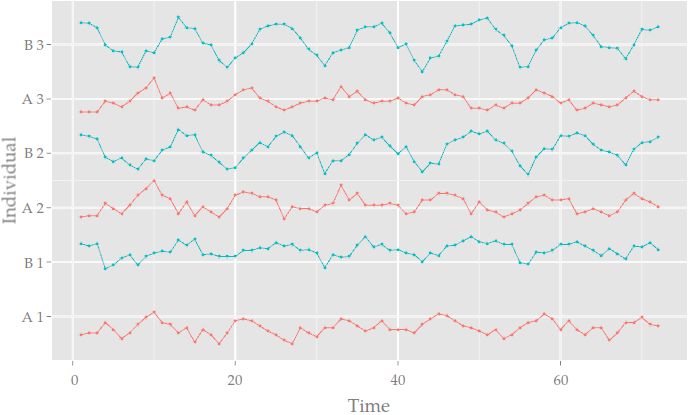
\includegraphics[width=0.48\textwidth]{graph/pipeline-14-7} & 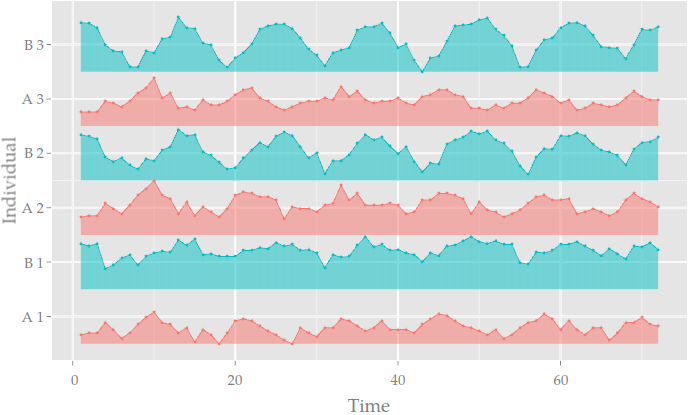
\includegraphics[width=0.48\textwidth]{graph/pipeline-14-9}\tabularnewline
\end{tabular}
\par\end{centering}

\caption{\label{fig:switching-layers}Switching between the line plot and the
area plot. The line plot is preferred in the first row for the compact
design without losing information. The area plot is preferred in the
second row for the easier comparison among values in different lines.}
\end{figure}



Switching between the layers does not change the data (just need to
add the baselines), but the following interactions will require for
some data modification.

\item Faceting.


Sometimes we care about some objects or time intervals more than others,
for instance, the patients under a special treatment, or the climate
observations in a year when the earthquakes frequently happened. In
other cases with many variables, we may have questions like whether
the variables share the same period? Do the peaks and valleys match
with each other? To explore the data with these questions, we need
to compare multiple time series.


In a static graph, several aesthetic methods can be used to distinguish
and compare multiple lines, like the color, size, or line type. However,
the aesthetic methods are not encouraged for a relatively large number
of lines, say, more than 10 lines. This is because the difference
of colors, sizes, or line types between adjacent lines could be too
weak to tell. Hence, faceting is considered as a technique to reduce
the number of lines displayed in the same region. Users can compare
within and between facet regions easily when the aspect ratio keeps
well.


There are three possible conditions to facet on: variable, individual
(for the longitudinal data), or period. Figure \ref{fig:faceting-var-ind}
gives an example for faceting on variable and individual. Design of
the faceting interaction should make the switching among five panels
done on-the-fly. Figure \ref{fig:faceting-period} explains why and
shows how to facet on period. Those faceting methods change the y-coordinates
of the points, and then the baselines of the area layer.


\begin{center}
\begin{figure}[H]
\begin{centering}
\begin{tabular}{cc}
\multicolumn{2}{c}{{\scriptsize{(a) not faceting}}}\tabularnewline
\multicolumn{2}{c}{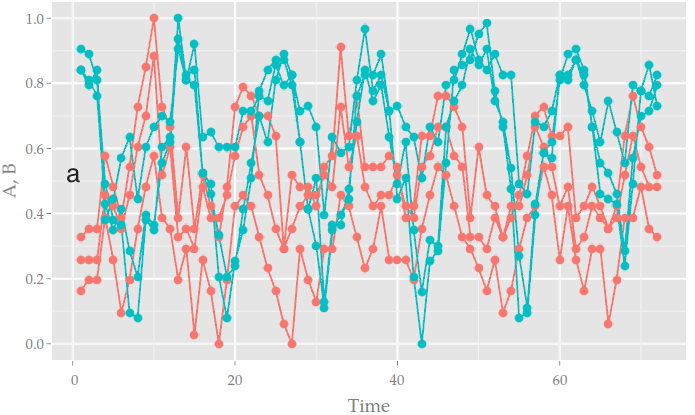
\includegraphics[width=0.48\textwidth]{graph/pipeline-14-1}}\tabularnewline
$\swarrow$ & $\searrow$\tabularnewline
{\scriptsize{(b) faceting by variable}} & {\scriptsize{(c) faceting by individual}}\tabularnewline
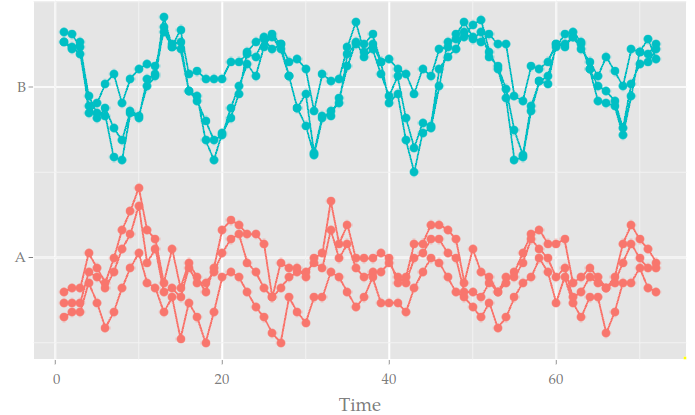
\includegraphics[width=0.48\textwidth]{graph/pipeline-14-2} & 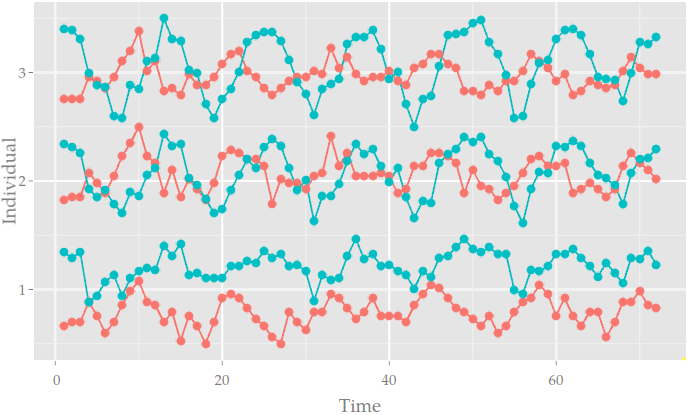
\includegraphics[width=0.48\textwidth]{graph/pipeline-14-3}\tabularnewline
$\downarrow$ & $\downarrow$\tabularnewline
{\scriptsize{(d) by variable then individual}} & {\scriptsize{(e) by individual then variable}}\tabularnewline
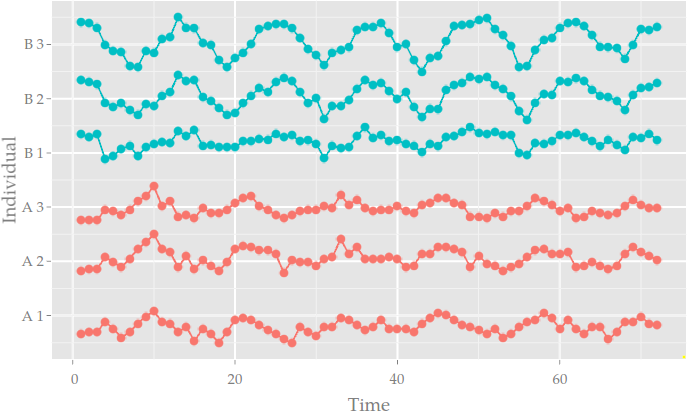
\includegraphics[width=0.48\textwidth]{graph/pipeline-14-4} & 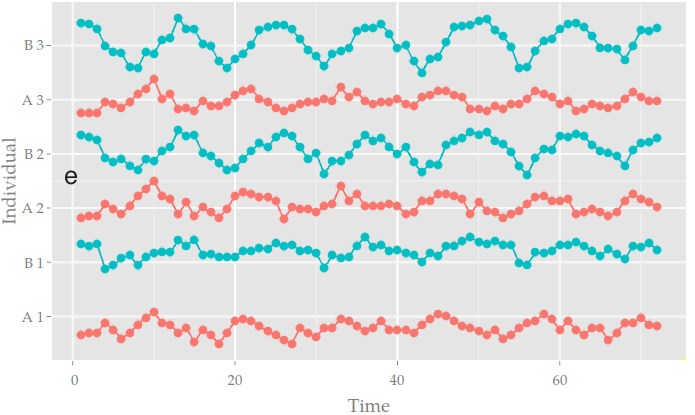
\includegraphics[width=0.48\textwidth]{graph/pipeline-14-5}\tabularnewline
\end{tabular}
\par\end{centering}

\caption{\label{fig:faceting-var-ind}Faceting on a longitudinal data set with
two variables and three individuals. (a) is the original plot with
six lines mixed. (b) splits the lines into two groups for two variables.
(d) follows the faceting from (b) then separates the three lines in
each group. (c) is another way of faceting where three individuals
are separated. (e) disperses the variables for each individual in
(c).}
\end{figure}

\par\end{center}


\begin{center}
\begin{figure}[h]
\begin{centering}
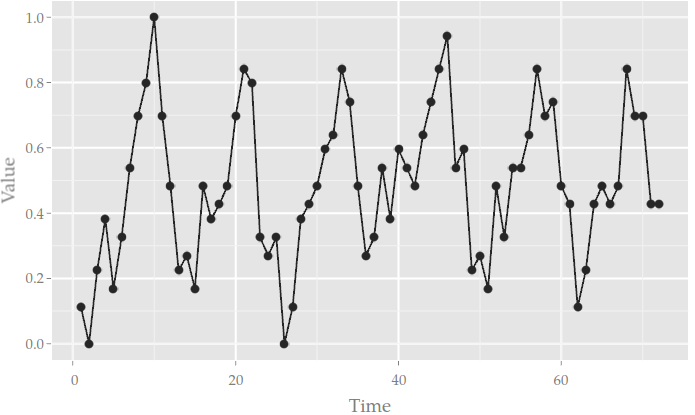
\includegraphics[width=0.32\textwidth]{graph/pipeline-01-1} 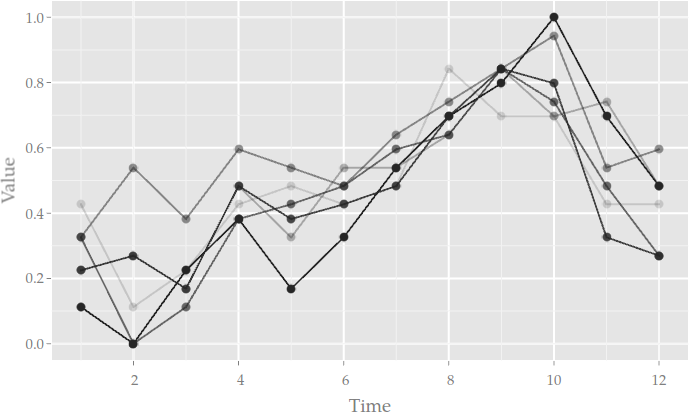
\includegraphics[width=0.32\textwidth]{graph/pipeline-15-5}
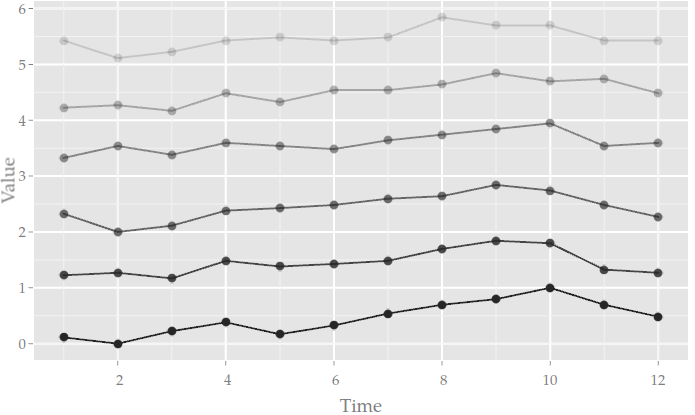
\includegraphics[width=0.32\textwidth]{graph/pipeline-15-3}
\par\end{centering}

\caption{\label{fig:faceting-period}An example of faceting on period for a
time series with a period of every 12 observations. The left panel
is the original series, the center and right panels show the periods
before and after faceting. From the left to center, the wrapping interaction
is used.}
\end{figure}

\par\end{center}


It is apparent that faceting by either variable, individual or both
helps to find the similar or unusual temporal pattern among variables
and individuals. To realize this functionality we use the variables
as the y input, and specify the variable name that indicates the individuals
or groups. Faceting on period is similar as faceting on individual
-- in both ways the observations are grouped by a variable indicator
and the points within group are connected. One idea is that if the
faceting-on-period interaction can be substituted by faceting-on-individual,
to simplify the manipulation. If we treat the period as the individual,
then each period has one line of the same length, so we can plot them
together and use the individual faceting method to separate the lines.
But the answer is no. Two things are ignored in the idea. First, it
assumes that the period exists as a variable in the data, like the
year for monthly data. Second, it assumes that the time indexes for
each period are already the same. For example, in Figure \ref{fig:faceting-period}(left),
the time indexes for the original series are from 1-72. The indexes
for the six periods are 1-12, 13-24, 25-36, 37-48, 49-60, 61-72, respectively.
If we facet the period as faceting by individual, then the six lines
are separated vertically as well as horizontally, which is different
from Figure \ref{fig:faceting-period}(right). A necessary step for
faceting on period is to re-index the time points from the left panel
to the right. So it can not be replaced by faceting on individual.

\item Slicing and wrapping.


Slicing and wrapping cut the series by a fixed-length interval in
the horizontal/vertical direction, and shift the right/top pieces
to the left/bottom. It could change the x- / y- coordinates of the
data.


There are two reasons for slicing and wrapping. The first one is to
compare the periods, or to find the period for the data that is potentially
periodical. Also the periodic variation could be explored \citep{mcdonald1986periodic}.
For this purpose we suggest to wrap the series horizontally. Figure
\ref{fig:faceting-period}(left to center) gives an example of horizontal
wrapping with a known period. Figure \ref{fig:x-wrapping} shows an
example of wrapping process with an unknown period.


\begin{center}
\begin{figure}[h]
\begin{centering}
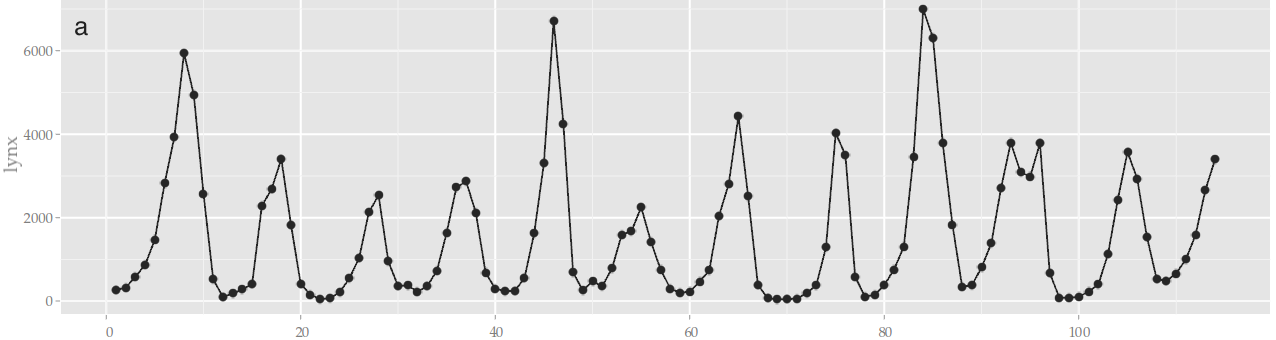
\includegraphics[width=0.98\textwidth]{graph/pipeline-16-original}
\par\end{centering}

\begin{centering}
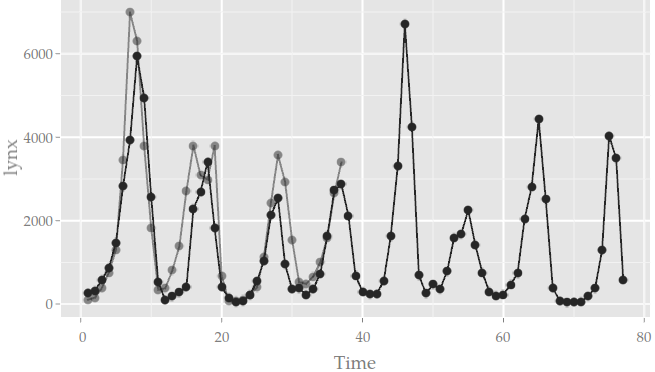
\includegraphics[width=0.48\textwidth]{graph/pipeline-16-1} 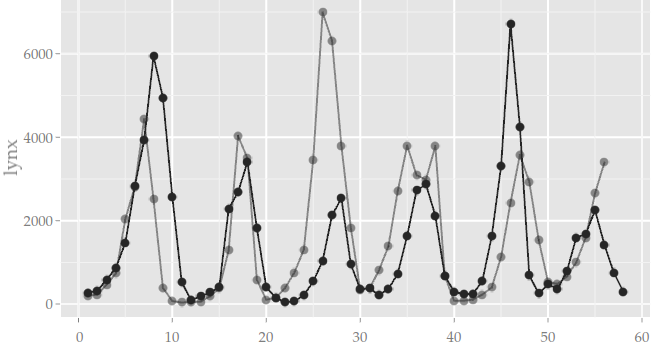
\includegraphics[width=0.48\textwidth]{graph/pipeline-16-2}
\par\end{centering}

\begin{centering}
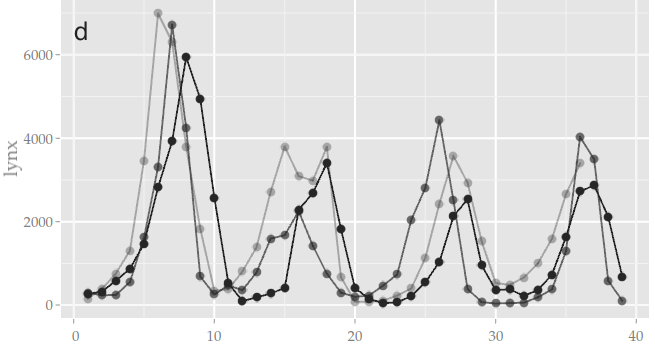
\includegraphics[width=0.48\textwidth]{graph/pipeline-16-xwrap} 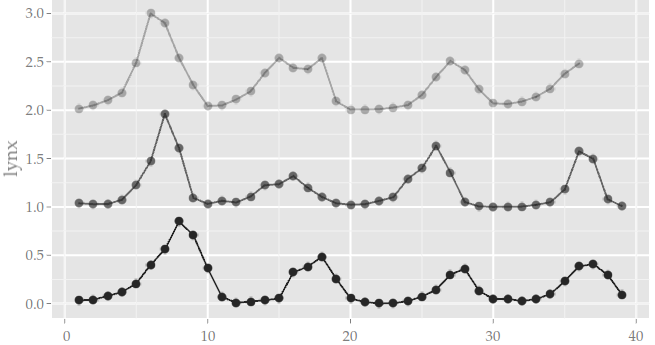
\includegraphics[width=0.48\textwidth]{graph/pipeline-16-xwrap-facet}
\par\end{centering}

\caption{\label{fig:x-wrapping}Top: time series plot of annual numbers of
lynx trappings for 1821\textendash{}1934 in the MacKenzie River District
\citep{campbell1977survey}. Second row: during the horizontal wrapping
movement, we try to match the late time period with the early time.
Bottom left: a good match of patterns usually indicates the potential
period. Bottom right: facet on the wrapped lines to view clearly.
Similar but not exactly matched pattern is seen here.}
\end{figure}

\par\end{center}


The second reason is to cut the temporal and longitudinal data into
parts for a better aspect ratio which will increase the effectiveness
of data display \citep{cleveland1987graphical}, and then reveal more
details. When the time series is long, to keep a proper aspect ratio
is not always workable, due to the the limit of the screen width.
Two possible solutions are (1) if the series is periodical, then wrap
it horizontally by the period, as Figure \ref{fig:faceting-period}
and \ref{fig:x-wrapping}. (2) Wrap the series vertically, especially
when multiple series are faceted.


Figure \ref{fig:y-wrapping} gives an example of the vertical wrapping
for quarterly pig production from 1967-1978 in United Kingdom \citep{andrews1985data}.
The four variables are HERDSZ: actual breeding herd size, PRODUCTION:
number of clean pig meat slaughtered, PROFIT: ratio of all-pig price
to all fattener feed price, GILTS: number of sows in pig for the first
time. In the top panel we see some overall pattern but it is hard
to compare two values from the first quarter and last quarter of a
line. In the bottom panel the series are wrapped in an area plot.
The darkness of the colors indicates the magnitude of the series values,
and the color bands make the comparison within or between the series
much easier. 


\begin{center}
\begin{figure}[h]
\begin{centering}
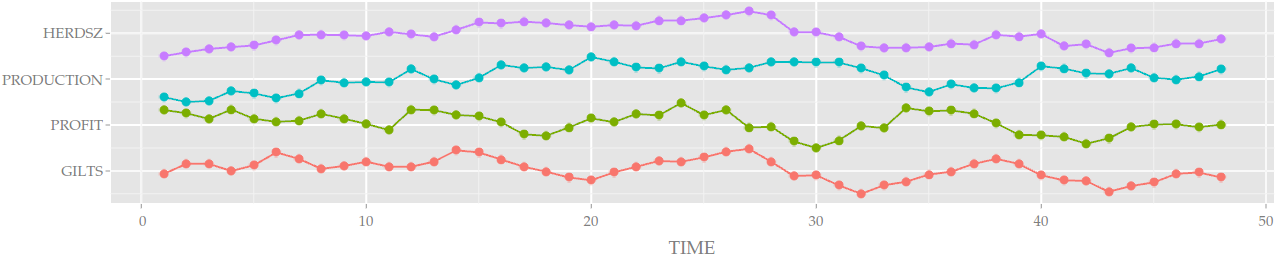
\includegraphics[width=0.98\textwidth]{graph/pipeline-17-original-wp-l}
\par\end{centering}

\begin{centering}
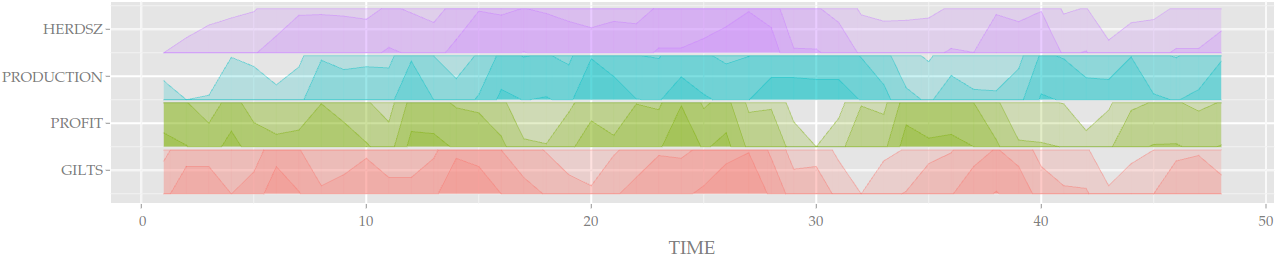
\includegraphics[width=0.98\textwidth]{graph/pipeline-17-ywrap-w}
\par\end{centering}

\caption{\label{fig:y-wrapping}Quarterly pig production for 1967-1978 in UK.
Top: the original data faceted on variable. HERDSZ and PRODUCTION
goes up slowly then down after the midway, and grows a little at the
end. PROFIT and GILTS seems to show the seasonality with increasing
variation. Bottom: wrapping in y-direction. We see the gradually change
for the first two variables and seasonal change for the latter two
variables, also a leading pattern between PROFIT and GILTS.}
\end{figure}

\par\end{center}

\item Mirroring.


Mirroring is an interaction proposed by the horizon graphs that helps
to compare the extreme values of the two sides, save more room for
the main body, and provide a better display for the series with binary
features like loss and earning. It dichotomizes the series by a horizontal
divider and reflects the bottom area up to the divider with a change
of the color scheme. The y-coordinates of the data are modified by
this interaction.


Figure \ref{fig:mirroring} shows the mirroring result for the lynx
trappings data with the mean divider. From the mirrored plot we see
the peaks last shortly but are sharp and irregular, the valleys are
smooth and regular.


\begin{center}
\begin{figure}[h]
\begin{centering}
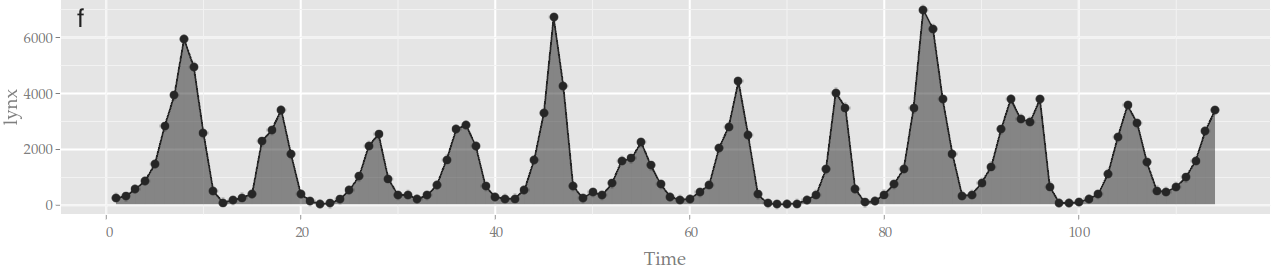
\includegraphics[width=0.98\textwidth]{graph/pipeline-18-original}
\par\end{centering}

\begin{centering}
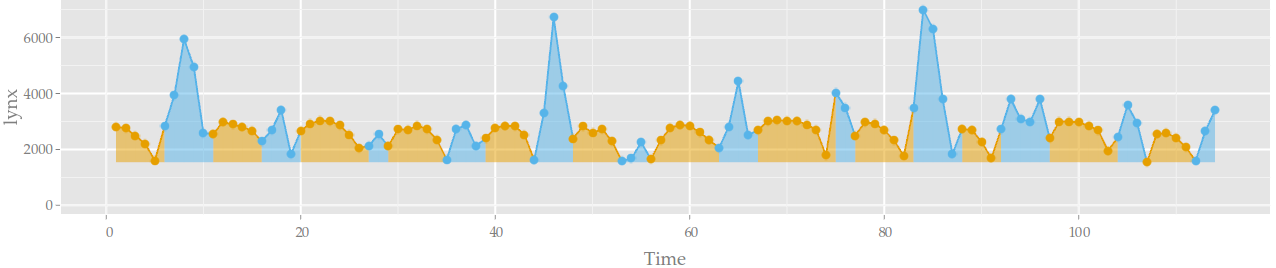
\includegraphics[width=0.98\textwidth]{graph/pipeline-18-mirrored}
\par\end{centering}

\caption{\label{fig:mirroring}Top: area plot for the lynx trappings data.
Bottom: mirroring by the mean. Two colors are assigned to the upper
and lower part: blue are the values above the mean, yellow below the
mean.}
\end{figure}

\par\end{center}


\begin{flushleft}
However, two issues raise up during the mirroring process: (1) how
to choose the horizontal divider -- midpoint of the range, mean of
the series, or the initial value? For the financial related data,
the starting value is preferred, like the price when entering the
market. But for other types of time series, the choice would depend
on the research interest. (2) when an edge crosses the divider, the
intersection will be a new data point to the line and need to be recorded.
The new data points could make problems, especially when other interactions
are added on the mirrored graph, like wrapping or linking. Section
\ref{sub:Linking-of-the-addition} introduces the problems from the
additional data in linking.
\par\end{flushleft}

\item Shifting.


When there are multiple series, we may consider to shift one or more
series horizontally to match with others for some reason, like the
starting time of the series is not the same, or one variable is leading
another. This interaction will modify the x-coordinates for the selected
series.


Figure \ref{fig:x-shifting} shows how shifting reveals the leading
pattern. From the left panel we see variable B (blue lines) has all
its pumps later than variable A (red lines), but we are not sure if
the lag is fixed or varied. So we can shift variable A to the right
by four time points and get the right panel. The peaks and valleys
match well for the two variables, which confirms the guess of leading
pattern.


\begin{center}
\begin{figure}[H]
\begin{centering}
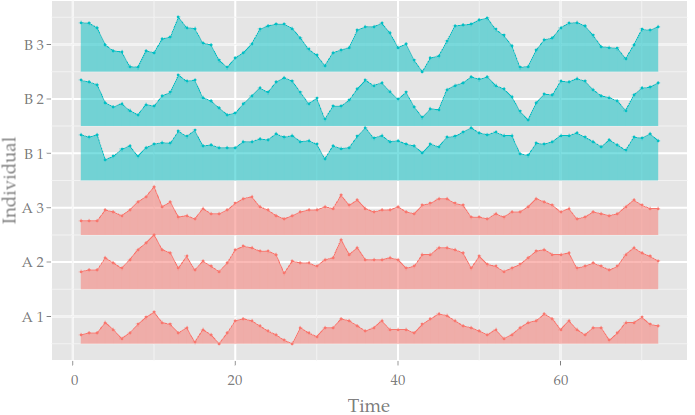
\includegraphics[width=0.48\textwidth]{graph/pipeline-19-original}
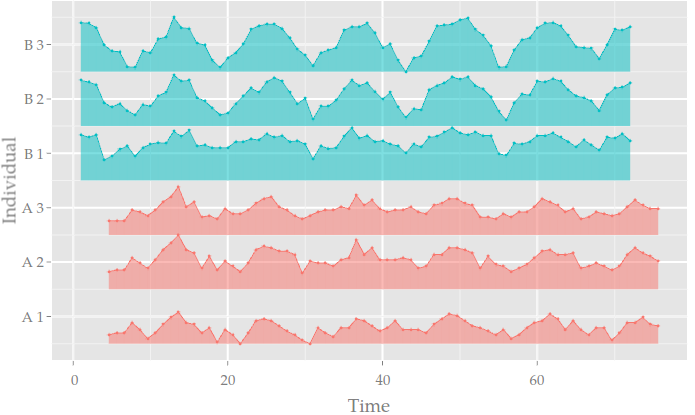
\includegraphics[width=0.48\textwidth]{graph/pipeline-19-shifting}
\par\end{centering}

\caption{\label{fig:x-shifting}Left: area plot for the longitudinal data with
two variables and three individuals. Right: three bottom lines from
variable A are shifted horizontally to the right, to match the peak
time with variable B.}
\end{figure}

\par\end{center}

\end{itemize}

\subsection{Discussion}


\subsubsection{Additivity\label{sub:Additivity}}

Summing up the common and special design together, there will be tens
of interactions for the temporal and longitudinal data. Most of them
are additive. That means interaction A can start at any status of
interaction B. For example, in Figure \ref{fig:faceting-var-ind},
if faceting on individual after faceting on variable, then the process
is in panel $(a\rightarrow b\rightarrow d)$, if faceting on variable
after individual, then it is $(a\rightarrow c\rightarrow e)$. In
Figure \ref{fig:faceting-period}, from the left to right, we experienced
horizontally wrapping and faceting by period, similar as Figure \ref{fig:x-wrapping}.
If wrapping vertically after mirroring, the result will be a horizon
graph. Also, users should be able to select the points, query the
information, and link to other graphs after any interaction.

To make the interactions additive is not trivial when the data coordinates
can be modified. It is not enough to know the current status, because
all of the special interactions are designed for two directions --
forward and backward. For the backward interactions, we need to know
when to stop, i.e., the initial status of the forward interactions.
Figure \ref{fig:additive-interactions} explains why both the current
and initial status are required by a faceting example. Section \ref{sub:Two-procedures}
will introduce the ways to store the initial and current status.

\begin{center}
\begin{figure}[h]
\begin{centering}
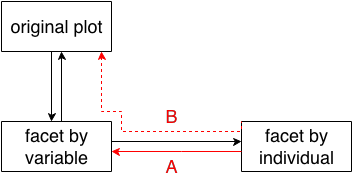
\includegraphics[width=0.5\textwidth]{graph/pipeline-20-additive-interactions}
\par\end{centering}

\caption{\label{fig:additive-interactions}A diagram of the additive interactions.
From the original plot we can facet the series by variable and mix
them back to the original picture. From the plot faceted by variable
we can conduct a second faceting by individual. Then the mixing of
individuals may lead to two positions by process A and B. Process
A takes the plot back to the end of the first faceting and the beginning
of the second faceting. Process B does not stop when the individuals
are mixed, but keeps working until all the lines are mixed, since
mixing is just the change of y-coordinates towards the initial location.
To avoid process B, the status of faceting by variable should be marked
and saved.}
\end{figure}

\par\end{center}


\subsubsection{Transfer speed}

For the interactions that modify the data coordinates, there will
be a starting position, several (or none) intermediate positions and
a target position (Figure \ref{fig:smoothness}). The starting position
is the point coordinates before the interaction. The target position
is the coordinates that maximize the effect of the interaction. The
target position could either be known or unknown by the user. When
it is known, any intermediate positions are not urgently needed, the
interaction could be just a command to make the points jump from the
starting position to the target. For example, with a known period,
the user can wrap the series on the period directly. However, under
many situations the target position is not known, and human intelligence
are involved to seek the target. Then the intermediate positions are
very important, and the step length between intermediate positions
is crucial. The small steps make the interaction look smooth and not
likely to miss the interesting phenomena, but are slow to reach the
optimum. The big steps get close to the target quickly, but may miss
it. Hence a gear to adjust the step length will be handy to control.

\begin{center}
\begin{figure}[h]
\begin{centering}
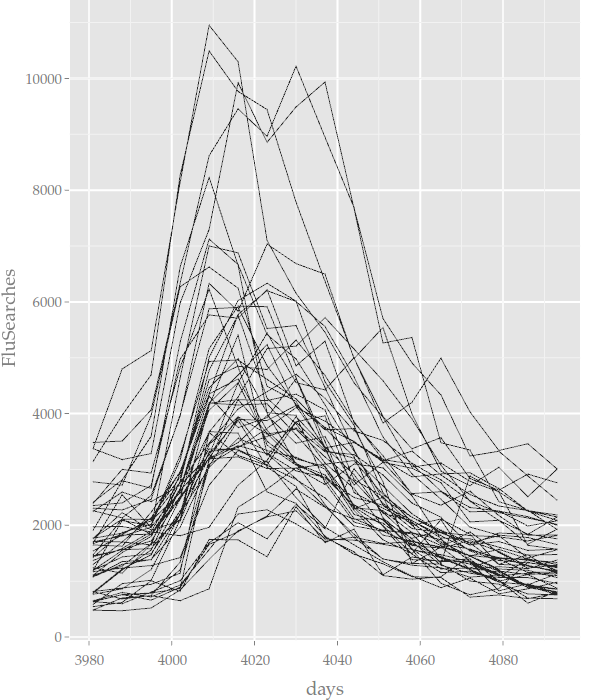
\includegraphics[width=0.32\textwidth]{graph/pipeline-22-original}
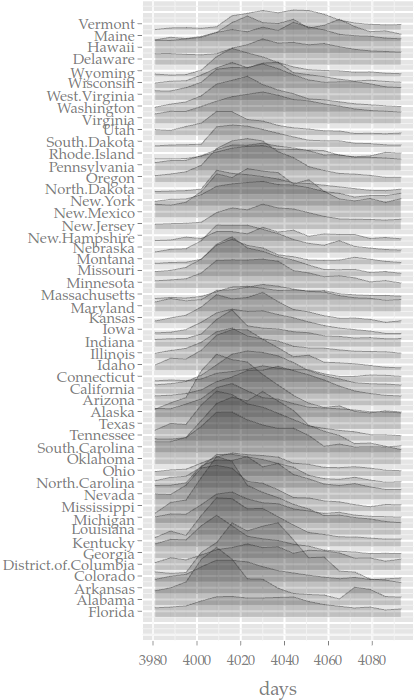
\includegraphics[width=0.32\textwidth]{graph/pipeline-22-smooth}
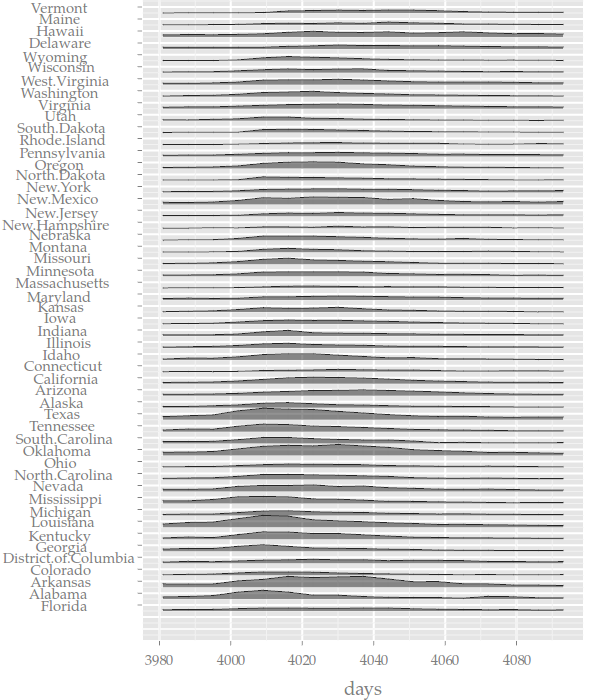
\includegraphics[width=0.32\textwidth]{graph/pipeline-22-jump}
\par\end{centering}

\caption{\label{fig:smoothness}Three positions of the faceting. Left panel
is the starting position, center is an intermediate position with
area layer, and right is the target position.}
\end{figure}

\par\end{center}


\subsubsection{Bi-direction and loop}

Some interactions do not have an obvious target, for instance, changing
the step length between intermediate positions. Then two types of
designs for the movement direction are available, given by Figure
\ref{fig:interaction-direction}. The bi-direction design is smoother,
but there must exist two manipulating commands for the forward and
backward interactions. This is annoying to the users when there are
many interactions because it doubles the number of commands. The loop
design only needs one command, but a sudden change will happen in
the transition from the last position to the starting position. Also,
backing to the previous position will be a little painful by this
design.

\begin{center}
\begin{figure}[h]
\begin{centering}
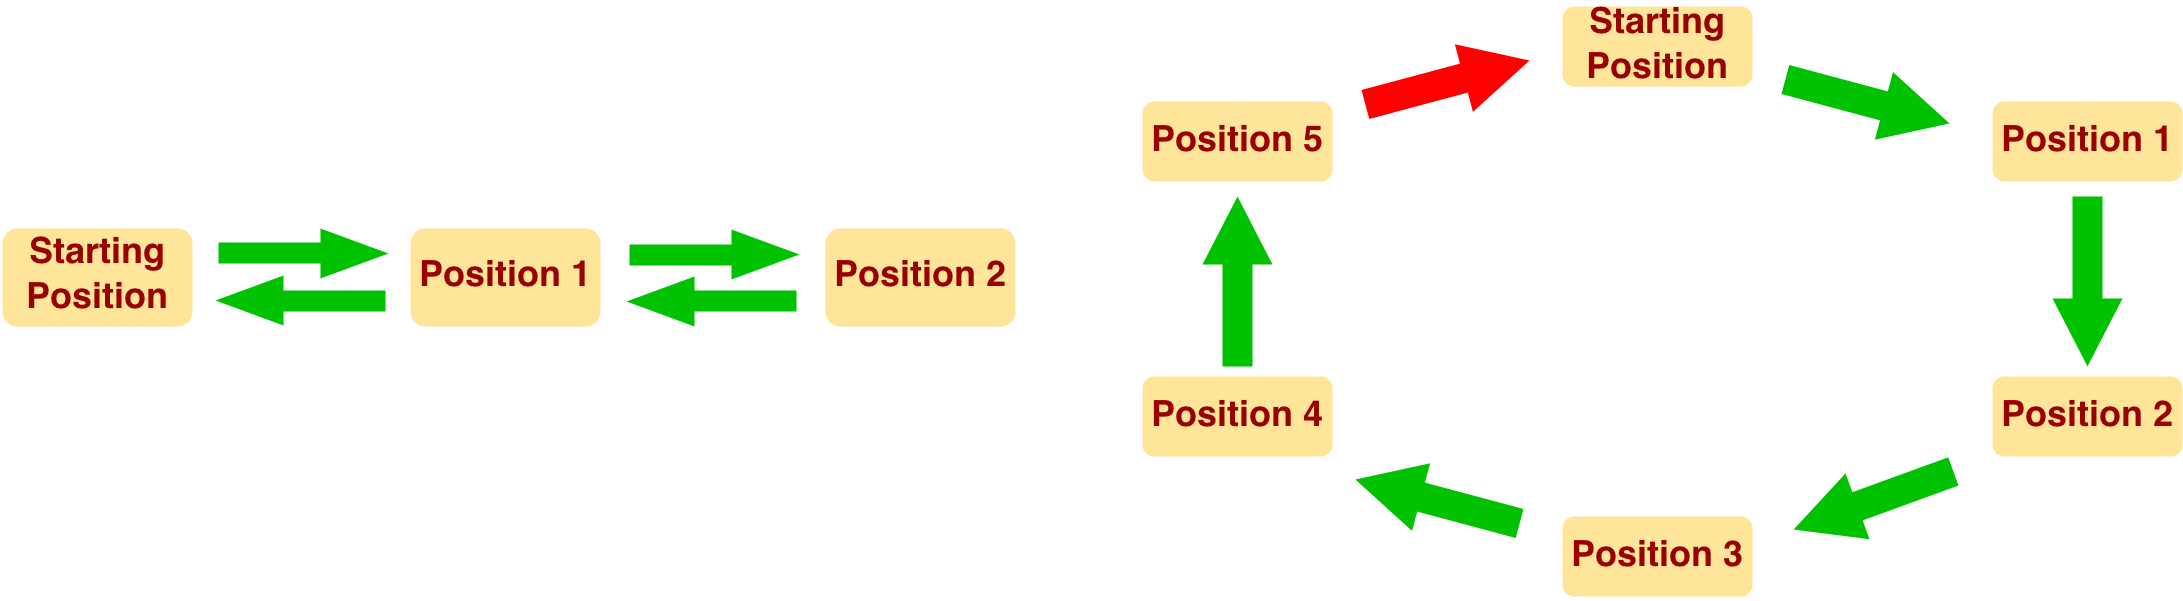
\includegraphics[width=0.98\textwidth]{graph/pipeline-21-directions}
\par\end{centering}

\caption{\label{fig:interaction-direction}Two designs for the direction of
interactions. Left panel is the bi-direction movement, and the right
panel is a loop.}
\end{figure}

\par\end{center}


\section{Display Pipeline\label{sec:Pipeline}}

\citet{wills2012visualizing} provided a basic equation for visualization
display as follows, and stated that the interactive graphics ``\textit{allow
the user to manipulate one of the two inputs, data or parameters,
and show the changes in the chart}''.

\[
data+parameters=graph
\]


This formula will be extended in this section, because in Will's equation,
$parameters$, including the element, aesthetic, coordinate, statistic,
scale, facet, and transform parameters, are too general to be well
defined. Moreover, most of the parameters that Will mentioned are
the graphical elements, like which elements to display, what color
scheme to use, etc. In a more specific interactive graphics design,
like the time series problem, the transform parameters need more attention.
Will did not give fully discussion for the last parameter type in
his book, but he pointed out that ``\textit{the transforms are strongly
data dependent}.'' In fact, the transformed data in the final display
also strongly depend on the transform parameters, when there exist
more than one type of transform. We will discuss how the interactions
change both the transform parameters and data as follows. Note that
the term $parameter$ will refer to the transform parameter, which
could change the coordinates of the data.


\subsection{Notations}

For each interaction, let $\mathbf{in}{}_{ij}^{T}=\left(in_{ij1},\, in_{ij2},\cdots\right)$
denote the user's input. Let $\mathbf{pa}{}_{i}^{T}=\left(pa_{i1},\, pa_{i2},\, pa_{i3},\cdots\right)$
be the corresponding parameter vector and $\mathbf{mv}{}_{ij}=\left(\Delta\mathbf{x}{}_{ij},\,\Delta\mathbf{y}_{ij}\right)$
denote the movements in x- and y- directions, where $i\in\mathcal{I}$
is an interaction type, $\mathcal{I}$ gives the temporal stream of
interaction types, such as $\{\textrm{faceting},\textrm{wrapping},\textrm{faceting},\textrm{zooming},\cdots\}$,
and $j=1,2,\cdots,n_{i}$ is the times of interactions under type
$i$.
\begin{lyxlist}{00.00.0000}
\item [{Example}] in Figure \ref{fig:smoothness}, the interaction type
$i=$ faceting. The center panel is triggered by pressing key U for
three times from the left panel, so for the center panel $j=3$. The
right panel appears after hitting key U for at least 20 times from
the left panel, so $j\geq20$. The number 20 is got by the initial
setting of the parameter $pa_{i1}=0.05$, which means that every hit
on key U will lift the $k$th standardized line by $(k-1)\times0.05$.
Hence for $i=$ faceting and $j\in\mathcal{N}$,
\begin{eqnarray*}
\mathbf{mv}{}_{ij} & = & \begin{cases}
\left(0,\;0.05\,(k-1)\, j\right) & 1\leq j<20,\\
\left(0,\; k-1\right) & j\ge20.
\end{cases}
\end{eqnarray*}
We can also generalize the equation above by
\begin{eqnarray*}
\mathbf{mv}{}_{ij} & = & \begin{cases}
\left(0,\; pa_{i1}\,(k-1)\, j\right) & 1\leq j<\frac{1}{pa_{i1}},\\
\left(0,\; k-1\right) & j\ge\frac{1}{pa_{i1}},
\end{cases}
\end{eqnarray*}
where $pa_{i1}\in(0,1)$.
\end{lyxlist}
The example shows that $\mathbf{mv}{}_{ij}$ is a function of $\mathbf{pa}{}_{i}$,
$j$, and $\mathbf{k}_{ij}$, where $\mathbf{k}_{ij}=k$ in this example
means the line group indicator for faceting. Different interactions
may have different line group indicators, for example, wrapping chops
the series into a few lines, and the times of wrapping $j$ will determine
the line groups. Then the new data coordinates are given by 
\[
\left(\mathbf{x},\mathbf{y}\right)_{s+interaction_{ij}}=\left(\mathbf{x},\mathbf{y}\right)_{s}+\mathbf{mv}{}_{ij},
\]
where $s$ is the previous status before the interaction.

In some occasions $\mathbf{mv}{}_{ij}$ not only depends on $\mathbf{pa}{}_{i}$,
$j$, and $\mathbf{k}_{ij}$, but also the user input $\mathbf{in}{}_{ij}$.
Like shifting in Section \ref{sub:Special-interactions}, the user
can drag the series horizontally to any position. Then the direction
$(in_{ij1})$ and distance $(in_{ij2})$ dragged is the input from
the user. Hence we have
\[
\mathbf{mv}{}_{ij}=f_{i}\left(\mathbf{pa}{}_{i},\:\mathbf{in}{}_{ij},\;\mathbf{k}_{ij},\; j\right).
\]



\subsection{Two procedures\label{sub:Two-procedures}}

We will summarize two procedures to calculate the new data coordinates
after the interactions. The two methods respectively use the storage
on multiple copies of data, and a binding storage of the data and
movement.
\begin{enumerate}
\item Let


\begin{eqnarray*}
s_{0} & = & \textrm{initial status},\\
s_{t+1} & = & s_{t}+in_{i{\color{red}1}}.
\end{eqnarray*}
 Note that every new status is only one interaction after the previous
status. The coordinates are given by
\begin{eqnarray*}
\left(\mathbf{x},\mathbf{y}\right)_{s_{t+1}} & = & \left(\mathbf{x},\mathbf{y}\right)_{s_{t}}+\mathbf{mv}{}_{i1}\\
\mathbf{mv}{}_{i1} & = & f_{i}\left(\mathbf{pa}{}_{i},\;\mathbf{in}{}_{i1},\;\mathbf{k}_{i1}\right)
\end{eqnarray*}



This procedure always computes the next position directly from the
current position. The change only depends on the corresponding interaction
parameters and the input. The current status is stored in the memory
and ready to use for getting the next status. This method is an intuitive
design and widely used in the interactive graphs with few special
interaction types. For example, rotations by GGobi (\citealt{STLBC03})
could be either auto-oriented or user-oriented. Only the current position
of the data is stored and the next movement can be got easily from
the parameter setting and the user's input. The old positions are
not of interest during the rotation.


The advantage of this procedure includes the straightforward design,
and the convenience of moving to the previous or next status. However,
when there are many special interactions that could transform the
data, we need to record both the initial and current data positions
of each interaction type in the stream $\mathcal{I}$ (recall Section
\ref{sub:Additivity}). Then for an interaction stream $\mathcal{I}$
of length $l$, at least $l+1$ phases $\left(\left(\mathbf{x},\mathbf{y}\right)_{s_{0}},\left(\mathbf{x},\mathbf{y}\right)_{s_{t_{1}}},\left(\mathbf{x},\mathbf{y}\right)_{s_{t_{2}}}\cdots,\left(\mathbf{x},\mathbf{y}\right)_{s_{t_{l}}}\right)$
should be saved, where $t_{1},t_{2},\cdots,t_{l}$ are the time of
the end of interaction types $1,2,\cdots,l$. When the data set is
large, those copies will occupy too much memory. Also, the storage
and management of $\mathbf{in}{}_{i1}$'s and $\mathbf{k}_{i1}$'s
is often in a mess. Hence we considered the second procedure as follows.

\item In this method, to store the $l+1$ phases, we do not make $l+1$
copies of the data set, instead, the movement item is traceable. The
coordinates of any status can be computed by 
\begin{eqnarray*}
\left(\mathbf{x},\mathbf{y}\right)_{s_{t}} & = & \left(\mathbf{x},\mathbf{y}\right)_{s_{0}}+\sum_{i,j}\mathbf{mv}{}_{ij}\\
 & = & \left(\mathbf{x},\mathbf{y}\right)_{s_{0}}+\sum_{i,j}f_{i}\left(\mathbf{pa}{}_{i},\;\mathbf{in}{}_{ij},\;\mathbf{k}_{ij},\; j\right).
\end{eqnarray*}
Note that when a new position is required, the calculation starts
from the initial position instead of the previous status. The movements
from the original to the current position are computed instantly.


Now the problem turns to: how to store the movements? The answer is,
to save $\mathbf{k}_{ij}$ with the data. This is because $\mathbf{pa}{}_{i}$
is fixed and $j$ is known, but $\mathbf{in}{}_{ij}$ and $\mathbf{k}_{ij}$
are different by line, furthermore, $\mathbf{in}{}_{ij}$ would work
on $\mathbf{k}_{ij}$. So we need to know how the points are assigned
to the lines before calculating the movements. So the data frame that
we use to save the data includes not only the coordinates, point parameters
like size and color, but also the line group indicators $\mathbf{k}_{ij}$.


The advantage of this procedure is apparently that we do not have
to save multiple copies of data, and it is a better way to manage
the data and parameters during the interactions. However, we have
some concerns too. First, we assumed that the movements are additive.
This may not be always true, especially when the movement depends
on some midway data locations. Second, a fixed design of interactions
is preferred -- complex mixed movements will make it difficult to
get the overall change.

\end{enumerate}

\section{Linking\label{sec:Linking}}

Linking plays an important role in interactive graphics, since it
enhances the visualization of high dimensional data by highlighting
the same observations on different graphs. \citet{xie2014reactive}
introduced the mechanism and types of linking, and elaborated self-linking
and linking on different sources or aggregation levels. However, their
paper is limited to linking between the existing datasets. For the
temporal and longitudinal data, linking becomes more complicated when
there is the need for different forms of the dataset or additional
data. The two situations are discussed as follows.


\subsection{Linking between the time plot and other graphs}


\subsubsection{``wide data'' and ``long data'' }

The time series and longitudinal data are usually ``wide'', as for
each time point, there are inputs from multiple variables. To explore
the dependency of the variables regardless of the time, many graph
types, like the scatterplot and parallel coordinates plot, can be
applied. However, if we utilize the ``wide data'' directly to generate
a mutaframe and plot the time series, then different variables must
share the same point parameters as from the same observations, as
explained in Table \ref{tab:wide-data}.

It is not ideal to make all the dots upon the same time point look
the same. To force them to be brushed or unbrushed simultaneously
is even a worse design. Hence we need the ``long data'' to assign
different properties to different points. Table \ref{tab:long-data}
is the corresponding long data of Table \ref{tab:wide-data}.

\begin{center}
\begin{table}[h]
\begin{centering}
\begin{tabular}{c|ccc|ccc}
\hline 
\multicolumn{4}{c|}{Variables} & \multicolumn{3}{c}{Parameters}\tabularnewline
\hline 
Time & V1 & V2 & V3 & \texttt{.brushed} & \texttt{.color} & \texttt{.size}\tabularnewline
\hline 
1 & 3.1 & 27 & 11.9 & FALSE & red & 4\tabularnewline
2 & 3.4 & 23 & 12.5 & TRUE & blue & 3\tabularnewline
$\vdots$ & $\vdots$ & $\vdots$ & $\vdots$ & $\vdots$ & $\vdots$ & $\vdots$\tabularnewline
\hline 
\end{tabular}
\par\end{centering}

\caption{\label{tab:wide-data}An example of the ``wide data.'' For each
time point, the aesthetic parameters are shared by all the three variables.
When plotting the time series, the three dots at the same time point
will look exactly the same. If any value is brushed in another plot,
say if V1 at time 2 is brushed in a scatterplot, then \texttt{.brushed}
of time 2 turns TRUE, which will make V2 and V3 at time 2 brushed
too.}
\end{table}

\par\end{center}

\begin{center}
\begin{table}[h]
\begin{centering}
\begin{tabular}{c|cc|ccc}
\hline 
\multicolumn{1}{c}{} & \multicolumn{2}{c|}{} & \multicolumn{3}{c}{Parameters}\tabularnewline
\hline 
Time & Variable & Value & \texttt{.brushed} & \texttt{.color} & \texttt{.size}\tabularnewline
\hline 
1 & V1 & 3.1 & FALSE & red & 4\tabularnewline
\textcolor{red}{2} & \textcolor{red}{V1} & \textcolor{red}{3.4} & \textcolor{red}{TRUE} & \textcolor{red}{yellow} & \textcolor{red}{5}\tabularnewline
1 & V2 & 27 & FALSE & red & 4\tabularnewline
2 & V2 & 23 & FALSE & blue & 3\tabularnewline
1 & V3 & 11.9 & FALSE & red & 4\tabularnewline
2 & V3 & 12.5 & FALSE & blue & 3\tabularnewline
$\vdots$ & $\vdots$ & $\vdots$ & $\vdots$ & $\vdots$ & $\vdots$\tabularnewline
\hline 
\end{tabular}
\par\end{centering}

\caption{\label{tab:long-data}The corresponding ``long data'' of Table \ref{tab:wide-data}.
In this format we can change the parameters of one single dot, for
example, V1 at time 2. }
\end{table}

\par\end{center}

The long data is used for the time plot, but sometimes we still need
the wide data for the other plots, and want to link the time plot
with other plots. Hence the linking between two formats has to be
constructed.


\subsubsection{Linking between the ``wide data'' and ``long data''}

\citet{xie2014reactive} delineated how linking works for two data
objects. First a linking variable must be pointed out, then two listeners
are attached on the two objects. If the \texttt{.brushed} parameter
switches in one dataset, then the listener is triggered. And if any
observations from the second dataset have the same value in the linking
variable as the first dataset, then the corresponding \texttt{.brushed}
parameter in the second dataset will be changed. 

Note that the linking between wide data and long data is not a one-to-one
linking. In the direction from wide to long data, each entry in the
wide data can project to multiple entries in the long data. In the
other direction, an entry in the long data will map to one entry in
the wide data. The unbalanced linking could produce a problem, as
shown in Table \ref{tab:wide-long-linking}.

\begin{center}
\begin{table}[h]
\begin{centering}
\begin{tabular}{c|cc|ccc}
\multicolumn{1}{c}{} & \multicolumn{2}{c}{(a) Long data} & \multicolumn{3}{c}{}\tabularnewline
\hline 
Time & Variable & Value & \texttt{.brushed} & \texttt{.color} & \texttt{.size}\tabularnewline
\hline 
$\vdots$ & $\vdots$ & $\vdots$ & $\vdots$ & $\vdots$ & $\vdots$\tabularnewline
\textcolor{red}{2} & \textcolor{red}{V1} & \textcolor{red}{3.4} & \textcolor{red}{TRUE} & \textcolor{red}{blue} & \textcolor{red}{3}\tabularnewline
2 & V2 & 23 & FALSE & blue & 3\tabularnewline
2 & V3 & 12.5 & FALSE & blue & 3\tabularnewline
$\vdots$ & $\vdots$ & $\vdots$ & $\vdots$ & $\vdots$ & $\vdots$\tabularnewline
\hline 
\end{tabular}
\par\end{centering}

\begin{centering}
$\Downarrow$
\par\end{centering}

\begin{centering}
\begin{tabular}{c|ccc|ccc}
\multicolumn{4}{c}{(b) Wide data} & \multicolumn{3}{c}{}\tabularnewline
\hline 
Time & V1 & V2 & V3 & \texttt{.brushed} & \texttt{.color} & \texttt{.size}\tabularnewline
\hline 
$\vdots$ & $\vdots$ & $\vdots$ & $\vdots$ & $\vdots$ & $\vdots$ & $\vdots$\tabularnewline
\textcolor{red}{2} & \textcolor{red}{3.4} & \textcolor{red}{23} & \textcolor{red}{12.5} & \textcolor{red}{TRUE} & \textcolor{red}{blue} & \textcolor{red}{3}\tabularnewline
$\vdots$ & $\vdots$ & $\vdots$ & $\vdots$ & $\vdots$ & $\vdots$ & $\vdots$\tabularnewline
\hline 
\end{tabular}
\par\end{centering}

\begin{centering}
$\Downarrow$
\par\end{centering}

\begin{centering}
\begin{tabular}{c|cc|ccc}
\multicolumn{1}{c}{} & \multicolumn{2}{c}{(c) Long data} & \multicolumn{3}{c}{}\tabularnewline
\hline 
Time & Variable & Value & \texttt{.brushed} & \texttt{.color} & \texttt{.size}\tabularnewline
\hline 
$\vdots$ & $\vdots$ & $\vdots$ & $\vdots$ & $\vdots$ & $\vdots$\tabularnewline
\textcolor{red}{2} & \textcolor{red}{V1} & \textcolor{red}{3.4} & \textcolor{red}{TRUE} & \textcolor{red}{blue} & \textcolor{red}{3}\tabularnewline
\textcolor{red}{2} & \textcolor{red}{V2} & \textcolor{red}{23} & \textcolor{red}{TRUE} & \textcolor{red}{blue} & \textcolor{red}{3}\tabularnewline
\textcolor{red}{2} & \textcolor{red}{V3} & \textcolor{red}{12.5} & \textcolor{red}{TRUE} & \textcolor{red}{blue} & \textcolor{red}{3}\tabularnewline
$\vdots$ & $\vdots$ & $\vdots$ & $\vdots$ & $\vdots$ & $\vdots$\tabularnewline
\hline 
\end{tabular}
\par\end{centering}

\caption{\label{tab:wide-long-linking}Linking between the long and wide data
may produce a problem. Suppose we start from brushing a point (V1
at time 2) in the long data (a). Then the listener of the long data
is triggered and changes the .brushed parameter for time 2 in the
wide data (b). Then the listener of the wide data is triggered and
switches the .brushed parameter for all the observations at time 2
in the long data (c), which conflicts with (a).}
\end{table}

\par\end{center}

The way to solve this problem is cutting off the backward linking.
To facilitate the cutoff, we can make a trick when adding the listeners
to the datasets. We put two signals in the two listeners. When one
listener is triggered, the signal will be turned on until the listener
finishes its work. During this period, the other listener cannot work.
As in Table \ref{tab:wide-long-linking}, the arrow from (b) to (c)
will be cut off.


\subsection{Linking of the additional data\label{sub:Linking-of-the-addition}}

Besides the issue of wide data and long data, there are other datasets
created during the interactions, such as the follows.
\begin{itemize}
\item The polygon data from the area layer. 


As shown in Figure \ref{fig:three-layers}, the area layer does not
only need the values in the time series, but also the baseline to
form many polygons. To draw the polygons, the data must be rearranged
in an order of polygon vertexes. Each polygon is made of four vertexes:
two from the time series and two from the baseline. Because the polygon
layer should listen to the point and line layers, the link between
the original data and the polygon data is one-way.

\item Copies of the dataset during the first procedure in Section \ref{sub:Two-procedures}.


When adopting this procedure, the variations of original dataset will
be created with multiple stages of the interactions. However, these
additional datasets are not required to get linked, because we only
make the copies of the coordinates, not the properties. To use the
coordinates, we combine them with the properties in the last minute,
so there will not be any linking issues.

\item Additional areas from the vertical slicing.


The example of vertical slicing is shown in Figure \ref{fig:y-wrapping}
and Figure \ref{fig:Additional-data} explained how the interaction
creates the additional areas. In Figure \ref{fig:Additional-data},
the black dots are given by the time series, and the red dots are
created during the slicing, by the choice of cutting lines. The black
and red dots are mixed in some order to form the shaded polygons.
Whenever a point is brushed, one, two, or even more sliced polygons
should be highlighted. Hence the two-direction linking between the
sliced polygons and points should be constructed. Note that this is
a one-to-$n$ mapping, and the linking variable is the point ID, which
should be assigned to the polygons when the red dots are generated.


\begin{center}
\begin{figure}[h]
\begin{centering}
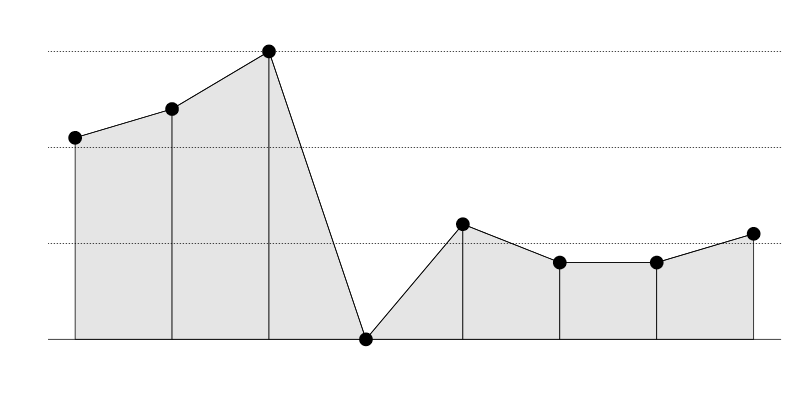
\includegraphics[width=0.48\textwidth]{graph/pipeline-23-1} 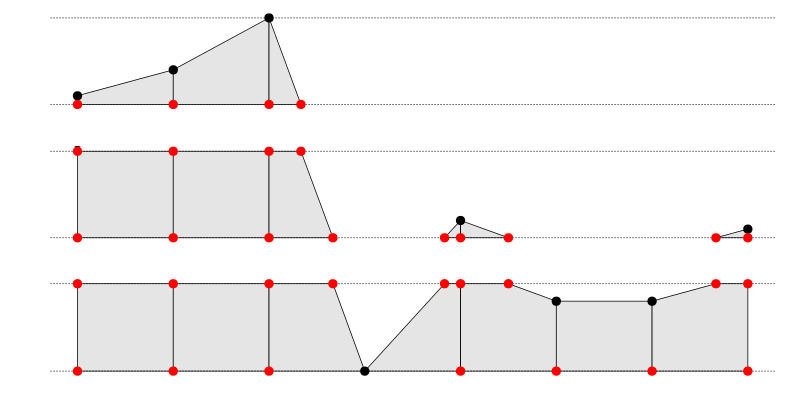
\includegraphics[width=0.48\textwidth]{graph/pipeline-23-2}
\par\end{centering}

\caption{\label{fig:Additional-data}Additional data created from the vertical
slicing. The black dots are given by the time series, and the red
dots are created during the slicing.}
\end{figure}

\par\end{center}

\end{itemize}

\section{Conclusion}

In this paper we reviewed the static and interactive graphics for
the time series and longitudinal data and refined the types of interactions.
For the time dependent data, several issues for the interactive design
(three layers, four interactions, two pipeline procedures, and linking)
are elaborated. However, some issues are still open to further discussion,
like the additivity, transfer speed, and the interaction direction.
Also, more special interactions would be needed for the time dependent
data in future, though they may bring new problems.

This paper aims at the time series and longitudinal data, but the
ideas on how to design and integrate good interactions can be applied
to other interactive graphics too.

\bibliographystyle{apa}
\bibliography{cranvastime}

\end{document}
